\documentclass[a4paper]{article}

\usepackage[utf8]{inputenc}
\usepackage[T1]{fontenc}
\usepackage{textcomp}
\usepackage[dutch]{babel}
\usepackage{amsmath, amssymb}
\usepackage[]{float}
\usepackage[margin = 3 cm]{geometry}
\usepackage{tikz}
\usepackage{physics}
\tikzset{>=latex} % for LaTeX arrow head
\usepackage{xcolor}
\definecolor{myblue}{HTML}{6272A4}
\definecolor{myred}{HTML}{44475A}
\definecolor{vcol}{HTML}{44475A}
\definecolor{EVcol}{HTML}{44475A}
\colorlet{Ecol}{orange!90!black}
\colorlet{Bcol}{violet!90}

% figure support
\usepackage{import}
\usepackage{xifthen}
\pdfminorversion=7
\usepackage{pdfpages}
\usepackage{transparent}
\newcommand{\incfig}[1]{%
	\def\svgwidth{\columnwidth}
	\import{./figures/}{#1.pdf_tex}
}

\pdfsuppresswarningpagegroup=1

\begin{document}
\begin{center}
	\begin{Huge}
	Problem 07 : : 	PHYS 201
	\end{Huge}
	\begin{Large}
		Ahmed Sabit (ass15)
	\end{Large}
\end{center}
\vspace{2cm}
\section*{Problem 1} 

The amplitude is given by the equation 
\[
E(r,t) = \frac{E_m}{r} \sin\left(kr \pm \omega t\right)
\] 
The wave equation in three dimensions is given by 
\[
\frac{\partial ^2 \psi}{\partial t ^2} = c^2 
\nabla ^2 \psi
\]
In spherical coordinates we have the re-written equation 
\[
	\frac{\partial ^2 \psi}{\partial t^2} 
	=
c^2 \frac{1}{r^2} \frac{\partial}{\partial r} \left(r^2 \frac{\partial \psi}{\partial r}\right)
\] 
Solving for the given equation of electric field \textbf{Left Side}
\begin{align*}
\frac{\partial ^2 E(r,t)}{\partial t ^2} = 
-\omega^2 \frac{E_m}{r} \sin(kr \pm \omega t )
\end{align*}
Solving for the \textbf{Right Side}
\begin{align*}
c^2	\frac{1}{r^2} \frac{\partial}{\partial r} 
	\left(r^2 \frac{\partial E(r,t)}{\partial r}\right) &= c^2
\frac{1}{r^2} \frac{\partial }{\partial r} 
\left(
r^2 \cdot  \left[
- \frac{E_m}{r^2} \sin\left(kr \pm \omega t\right) + k \frac{E_m}{r} \cos 
\left(kr \pm \omega t\right)
\right]
\right)
	\\
							    &= c^2
\frac{1}{r^2} \frac{\partial }{\partial r} 
\left(
- {E_m} \sin\left(kr \pm \omega t\right) + kr {E_m} \cos 
\left(kr \pm \omega t\right)
\right)
	\\
							    &= c^2
\frac{1}{r^2} 
\left(
- k {E_m} \cos \left(kr \pm \omega t\right) + 
k {E_m} \cos 
\left(kr \pm \omega t\right)
-
k^2r {E_m} \sin 
\left(kr \pm \omega t\right)
\right)
	\\
	&= 
- c^2 \frac{k^2 E_m}{r} \sin(kr \pm \omega t)
\\
&= 
- \omega^2 \frac{E_m}{r} \sin \left(kr \pm \omega t\right)
\tag{$c = \omega / k$ }
\\
\end{align*}
Woohoo we have both the left and right side equal. 
\[
c^2	\frac{1}{r^2} \frac{\partial}{\partial r}
	\left(r^2 \frac{\partial E(r,t)}{\partial r}\right) =
\frac{\partial ^2 E(r,t)}{\partial t ^2} = 
- \omega^2 \frac{E_m}{r} \sin \left(kr \pm \omega t\right)
\] 
This validates that the given equation $E(r,t)$ is an isotropic spherical wave solution.



\newpage
\section*{Problem 2} 
The electromagnetic wave in vacuum is given by (usual units)
\[
\vec{E} = 
\left({2}\right) 
\cos \left(
\omega \left(t - \frac{x}{c}\right)
\right) \hat{k}
\]
This is a great place to copy paste TiKZ code from the internet! We are going to draw a generic wave for this purpose. 

% Electromagnetic wave - colored
\begin{figure}[H]
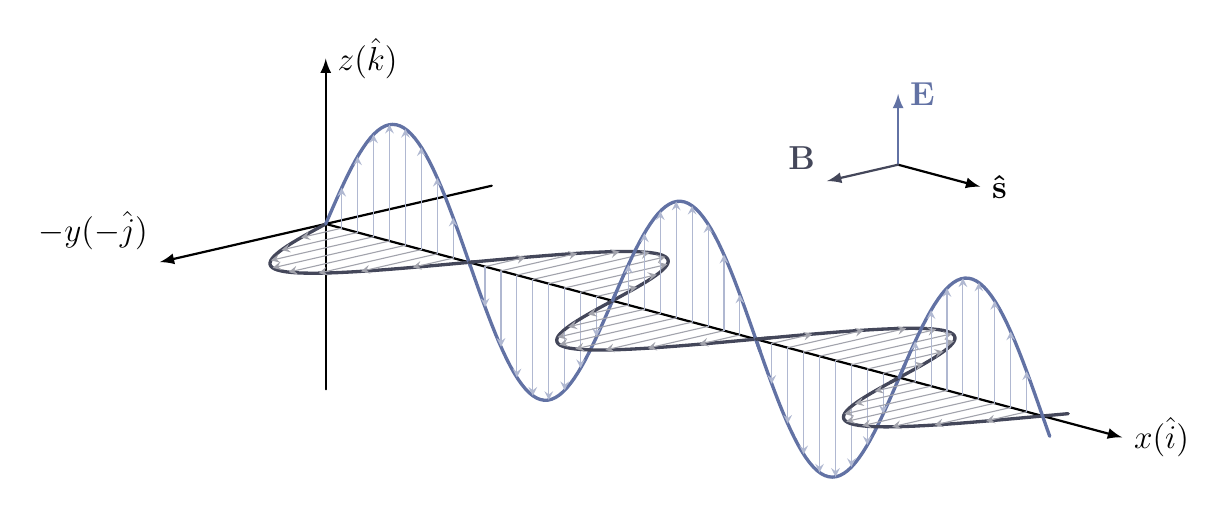
\begin{tikzpicture}[x=(-15:1.2), y=(90:1.0), z=(-150:1.0),
                    line cap=round, line join=round,
                    axis/.style={black, thick,->},
                    vector/.style={>=stealth,->}]
  \large
  \def\A{1.5}
  \def\nNodes{5} % use even number
  \def\nVectorsPerNode{8}
  \def\N{\nNodes*40}
  \def\xmax{\nNodes*pi/2*1.01}
  \pgfmathsetmacro\nVectors{(\nVectorsPerNode+1)*\nNodes}

  \def\vE{{\color{myblue}\mathbf{E}}}
  \def\vB{{\color{myred}\mathbf{B}}}
  \def\vk{\mathbf{\hat{k}}}

  \def\drawENode{ % draw E node and vectors with some offset
    \draw[myblue,very thick,variable=\t,domain=\iOffset*pi/2:(\iOffset+1)*pi/2*1.01,samples=40]
      plot (\t,{\A*sin(\t*360/pi)},0);
    \foreach \k [evaluate={\t=\k*pi/2/(\nVectorsPerNode+1);
                           \angle=\k*90/(\nVectorsPerNode+1);}]
                in {1,...,\nVectorsPerNode}{
      \draw[vector,myblue!50]  (\iOffset*pi/2+\t,0,0) -- ++(0,{\A*sin(2*\angle+\iOffset*180)},0);
    }
  }
  \def\drawBNode{ % draw B node and vectors with some offset
    \draw[myred,very thick,variable=\t,domain=\iOffset*pi/2:(\iOffset+1)*pi/2*1.01,samples=40]
      plot (\t,0,{\A*sin(\t*360/pi)});
    \foreach \k [evaluate={\t=\k*pi/2/(\nVectorsPerNode+1);
                           \angle=\k*90/(\nVectorsPerNode+1);}]
                in {1,...,\nVectorsPerNode}{
      \draw[vector,myred!50]  (\iOffset*pi/2+\t,0,0) -- ++(0,0,{\A*sin(2*\angle+\iOffset*180)});
    }
  }

  % MAIN AXES
  \draw[axis] (0,0,0) -- ++(\xmax*1.1,0,0) node[right] {$x(\hat{i})$};
  \draw[axis] (0,-\A*1.4,0) -- (0,\A*1.4,0) node[right] {$z (\hat{k})$};
  \draw[axis] (0,0,-\A*1.4) -- (0,0,\A*1.4) node[above left] {$-y (- \hat{j})$};

  % SMALL AXES
  \def\xOffset{{(\nNodes-2)*pi/2}}
  \def\yOffset{\A*1.2}
  \def\zOffset{\A*1.2}
  \draw[axis,black] (\xOffset,\yOffset,-\zOffset) -- ++(\A*0.6,0,0) node[right,align=center] {$\mathbf{\hat{s}}$}; %\\propagation
  \draw[axis,myblue]  (\xOffset,\yOffset,-\zOffset) -- ++(0,\A*0.6,0) node[right] {$\mathbf{E}$};
  \draw[axis,myred]   (\xOffset,\yOffset,-\zOffset) -- ++(0,0,\A*0.6) node[above left] {$\mathbf{B}$};

  % equation
%  \node[above right] at (\xOffset,-0.5*\yOffset,4*\zOffset)
%    {$\begin{aligned}
%		    \vE &= {\color{myblue}\mathbf{E_0}}\sin(\mathbf{\hat{s}}\cdot\mathbf{x}-c_0t)\\
  %    \vB &= {\color{myred} \mathbf{B_0}}\sin(\mathbf{\hat{s}}\cdot\mathbf{x}-c_0t)\\
  %    \end{aligned}$};
  %\node[below right] at (\xOffset,-0.5*\yOffset,4*\zOffset)
  % {$\vE\cdot\mathbf{\hat{s}} = 0,\;\; \vB\cdot\mathbf{\hat{s}} = 0,\;\; \vB = \frac{1}{c_0}\mathbf{\hat{s}}\times\vE$};
  % draw (anti-)nodes
  \foreach \iNode [evaluate={\iOffset=\iNode-1;}] in {1,...,\nNodes}{
    \ifodd\iNode \drawBNode \drawENode % E overlaps B
    \else        \drawENode \drawBNode % B overlaps E
    \fi
  }

\end{tikzpicture}
\end{figure}

Verification of the directions, we require the Poynting vector to point $+ x$ direction. 
\[
\vec{S} \propto \vec{E} \times \vec{B} \propto - \hat{z} \times \hat{y}   = 
\hat{x}
\] 
Validating $-y$ to be the direction where $\vec{B}$ points. 
\[
\vec{B} = 
\left(\frac{2}{c}\right)
\cos 
\left(
\omega 
\left(t - \frac{x}{c}\right)
\right) (- \hat{j})
\] 

\subsection*{(a)} 
The form is given by 
\[
\vec{B} = 
\left(\frac{2}{c}\right)
\cos 
\left(
\omega 
\left(t - \frac{x}{c}\right)
\right) (- \hat{j})
\] 
Where the amplitude is $B_0 = 6.67 \times 10^{-9} \, T$

\subsection*{(b)} 
Average intensity (as shown in EMWaves3.pdf lecture file) 
\[
S_\text{av} = \frac{E_m^2}{2 c \mu_0} = \frac{2}{c \mu_0} = 0.00530883746 \, W / m^2
\] 





\newpage
\section*{Problem 3} 
\subsection*{(a)} 
The magnetic field inside a long solenoid is given by 
\[
B_z = \mu_0 n i 
\]
So the magnetic field energy density is given by 
\[
u_B = \frac{\mu_0 n^2 i ^2}{2}
\]

\subsection*{(b)} 
Total energy inside the solenoid is given by 
\[
E = u_M V = \frac{\mu_0 n^2 i^2}{2} \pi r^2 l
\] 
The derivative is 
\[
\frac{\mathrm{d} E}{\mathrm{d}  t} = 
\mu_0 \pi r^2 n^2 l \left[i \frac{\mathrm{d} i}{\mathrm{d} t} \right] < 0 \impliedby \frac{\mathrm{d} i}{\mathrm{d} t} < 0 
\]
The overall power is negative. The energy is decreasing. Makes a lot of sense because $\frac{\mathrm{d} i}{\mathrm{d} t} $ is negative.  

\section*{(c)} 
We have linear $B$ field change because of changing current. Only taking account of magnitude and running down a computation of one of the Maxwell's equation
\[ E (2 \pi r) = 
\frac{\partial B}{\partial t} (\pi r^2)  \implies E = \frac{r}{2} \frac{\partial B}{\partial t}
\] 
$B$ and $i$ have linear dependence and because the above quantity is a derivative of $B$ only with respect to time, we have linear decrease of current that implies that Electric Field is going to be a constant in time. 

\subsection*{(d) + (e)} 
Power flowing through a theoretical cylinderical tube surface of radius $r$ inside the solenoid (of same length $l$) is computed. 
Total electromagnetic power is computed from the poynting vector
\[
S = \frac{EB}{\mu_0} = \frac{B}{\mu_0} \left( \frac{r}{2} \frac{\partial B}{\partial t}\right) = 
\frac{r}{2 \mu_0} \left(B \frac{\partial B}{\partial t}\right)
\] 
\[
	P = S A = S (2 \pi r l) = \left(\frac{r}{2 \mu_0} B \frac{\partial B}{\partial t} \right) 2 \pi r l = ( \pi r^2 l ) \frac{1}{\mu_0} B \frac{\partial B}{\partial t} = 
	\frac{\mathrm{d} }{\mathrm{d} t} \left(\text{(volume)} \frac{1}{\mu_0} \frac{B^2}{2}\right)
\]
Above its absolutely the same answer we got in the previous sections, just the derivative of energy lose. 
\begin{figure}[H]
	\centering
	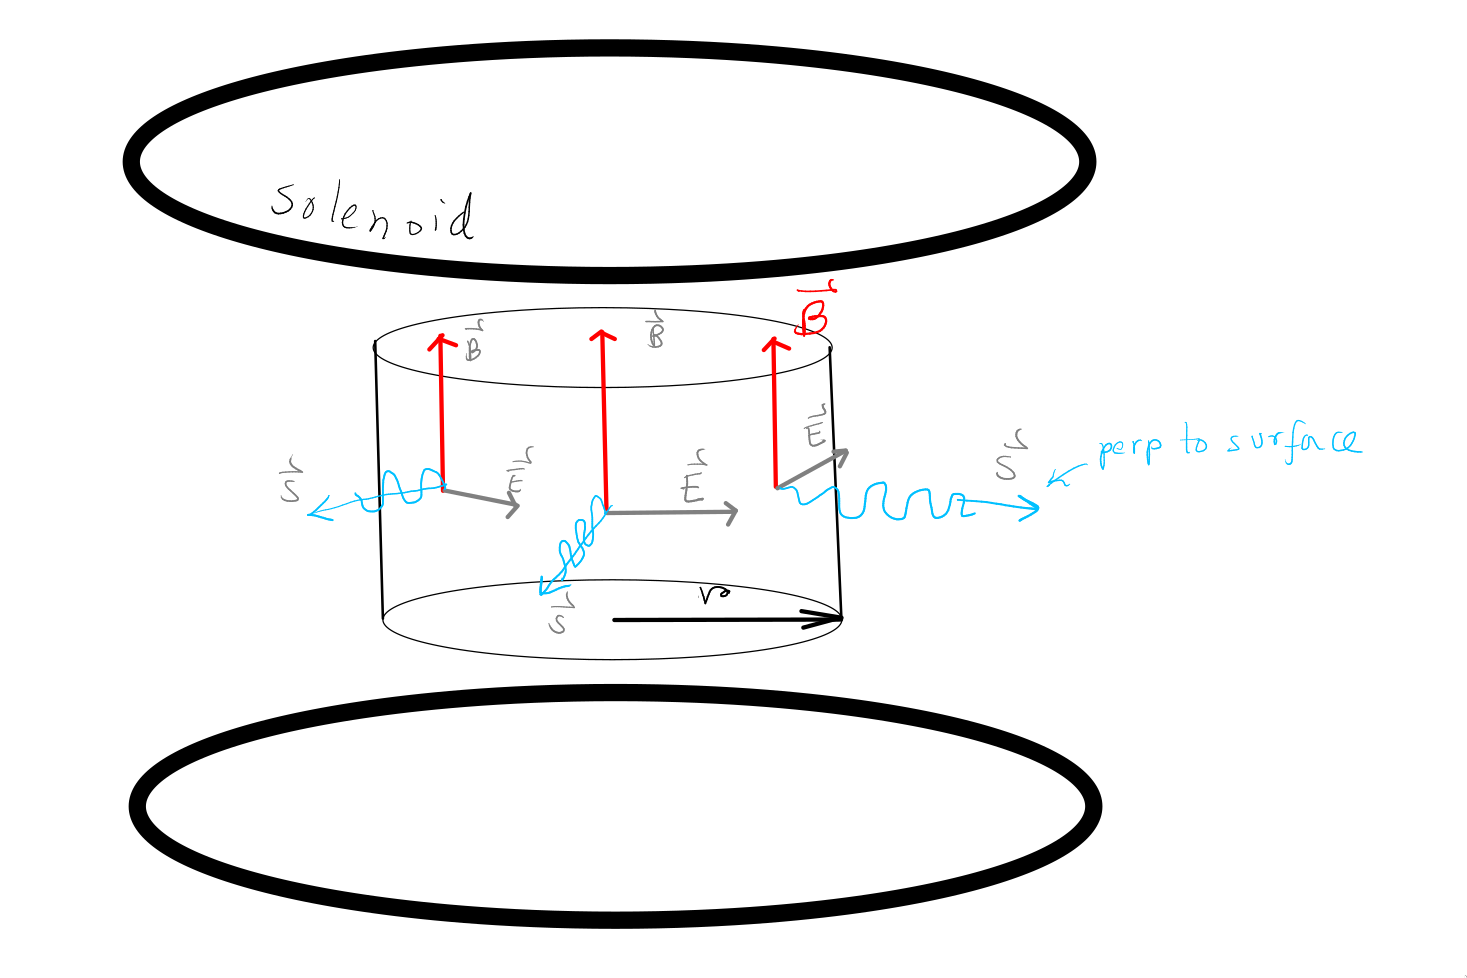
\includegraphics[width=0.8\textwidth]{./ss/7/1.png}
	\caption{Answer to  (d) in a sense, the Poynting vector points towards $\vec{E} \times  \vec{B}$}
	\label{fig:-ss-7-1-png}
\end{figure}
Hence total energy density inside the solenoid in terms of the magnetic field is 
\[
\frac{1}{2 \mu_0} B^2 
\] 
The electromagnetic radiation is also shown. 


\section*{Problem 4} 
\subsection*{(a)} 
\begin{align*}
	F &=  \frac{IA}{c} = \frac{PA}{A c} = \frac{P}{c}  \\
	&= \frac{1500}{c} = 5 \times 10^{6} 
\end{align*}
\begin{align*}
	a &= \frac{F}{m} = \frac{5 \times  10^{6}}{10 + 60} = 7.14 \times 10^{-8} 
\end{align*}
\[
20 = \frac{1}{2}at^2 \implies t = \sqrt{\frac{40}{a}}  = 23656 \, s  = 6.5 \text{ hours}
\] 
\[
\text{cannot make it in time}
\] 

\subsection*{(b)} 
Recompute the acceleration 
\[
a = \frac{F}{m} = 8.33 \times 10^{-8}
\] 
\[
t = \sqrt{\frac{40}{a}}  = 6.08 \text{ hours}
\] 
\[
\text{still does not make it. Sad. RIP.}
\] 

\subsection*{(c)} 
Using momentum conservation directly 
\[
0 = 60 v + 10 
\] 
Solving this gives with $t$ 
\[
t = 20 / (1 / 6) = 120 \, \text{s}
\]
\[
\text{this time yes, the time is enough}
\] 


\section*{Problem 5} 
\[
\cos a + \cos b = 
2 
\cos \left(\frac{a+b}{2}\right)
\cos \left(\frac{a-b}{2}\right)
\] 
\[
\sin a - \sin b = 
2 \cos \left(\frac{a+b}{2}\right)
\sin \left(\frac{a-b}{2}\right)
\] 
\subsection*{(a)} 
The superposition would be 
\begin{align*}
\vec{E}_R + 
\vec{E}_L &= 
\hat{i} 
\left(
E_m \cos(kz - \omega t) + E_m \cos(kz - \omega t + \phi_1)
\right)
\\
	  &+ \hat{j}
	  \left(
E_m \sin(kz - \omega t + \phi_1) - E_m \sin(kz - \omega t )
	  \right)
	  \\
	  & = 
	  2 E_m \cos \left( \frac{2(kz - \omega t) + \phi_1}{2}\right) 
	  \cos \left(- \frac{\phi_1}{2}\right) \hat{i} 
	  \\
	  & + 
	  2 E_m \cos \left(\frac{2 (kz - \omega t) + \phi_1}{2}\right)
	  \sin \left(\frac{\phi_1}{2}\right) \hat{j}
	  \\ & = 
	  2 E_m \cos \left( (kz - \omega t) + \frac{\phi_1}{2}\right) 
	  \cos \left( \frac{\phi_1}{2}\right) \hat{i} 
	  \\
	  & + 
	  2 E_m \cos \left( (kz - \omega t) + \frac{\phi_1}{2}\right)
	  \sin \left(\frac{\phi_1}{2}\right) \hat{j} 
	  \\
	  &= 
	  \left(2 E_m \cos \left(k z - \omega t + \frac{\pi}{6}\right)\right) 
	  \left[ \cos( \pi / 6) \hat{i} + \sin (\pi / 6) \hat{j} \right]
	  \\
	  &= 
	  \left(2 E_m \cos \left(k z - \omega t + \frac{\pi}{6}\right)\right) 
	  \left[ \frac{\sqrt{3} }{2}	\hat{i} + \frac{1}{2} \hat{j} \right]
	  \\
\end{align*}
The wave can be thought of as going along the $\sqrt{ 3}  \hat{i} + \hat{j}$ direction with a wave form given by the bracketed thing in the left. This is proven to be linearly polarized
\[
\psi(z,t) = 2 E_m \cos ( k z - \omega t + \pi / 6)
\]
This makes $\pi / 6 \text{ rad}$ angle with the $\hat{x}$ axis.

\subsection*{(b)} 
\[
S_\text{av} = \frac{E^2}{2 c \mu_0} = \frac{2 E_m ^2}{c \mu_0}
\]

\subsection*{(c)} 
It's only the $y$ component that passes through. 
\[
S_\text{y, av} / S_\text{av} = E_\text{y,m}^2 / E_m^2 = (1 / 2)^2 = \frac{1}{4}
\] 

\subsection*{(d)} 
\[
E_R = \frac{(-E_m)^2}{E_m^2} = 1
\] 
\[
E_L = \frac{E_m ^2 \sin ^2 \phi_1}{E_m ^2} = \sin ^2 \phi_1 = 0.75
\] 

\section*{Problem 06} 
\begin{align*}
	I_1 &= I_0 \cos ^2 (\theta_1 - \theta_0) \\
	I_2 &= I_0 \cos ^2 (\theta_2 - \theta_1) \cos ^2 (\theta_1 - \theta_0) \\
	    & \vdots \\ 
	I_n &= I_0 (\cos ^2 \Delta \theta)^{n} \tag{$\Delta \theta = \theta_2 - \theta_1 = \theta_1 - \theta_0 $ } \\
	I_3 &= I_0 \cos^{6} (\pi / 6) = 0.42 I_0 \\
	I_6 &= I_0 \cos^{12}(\pi / 12) = 0.66 I_0 \\
	I_9 &= I_0 \cos^{18} (\pi /18) = 0.76 I_0 \\
	I_{90} & \approx 0.97 I_0 \tag{using relevant approximations}
\end{align*}
We get the Highest for $9$ filters. 


\section*{Problem 7} 
\subsection*{(a)} 
The form could be written as
\[
\vec{E} = 
\vec{E}_0 \sin \left(\frac{m \pi x}{L}\right)
\sin \left(\frac{n \pi y}{L}\right)
\sin \left(\frac{p \pi z}{L}\right) 
\cos \left(t \frac{\pi c}{L} \sqrt{m^2 + n^2 + p^2} \right)
\] 

\subsection*{(b)} 
First harmonic is $m = p = n = 1$ which gives $\lambda = 2L = 50 cm$

\subsection*{(c)} 
\[
f= \frac{c}{\lambda} \sqrt{m^2 + n^2 + p^2} 
\] 

\subsection*{(d)} 
\begin{align*}
	(m,n,p ) = (1,1,1) &\implies f_1 = \frac{c}{\lambda} \sqrt{3}  = 1.03 \times 10^{4} \, \text{Hz} \\ 
	(2,1,1) &\implies f_2 = \frac{c}{\lambda} \sqrt{6}  = 1.46 \times 10^{4} \, \text{Hz} \\ 
	(2,2,1) &\implies f_3 = \frac{c}{\lambda} \sqrt{9}  = 1.74 \times 10^{4} \, \text{Hz}
\end{align*}
\end{document}
